\documentclass[a4paper]{article}

\usepackage[a4paper,margin=2cm]{geometry}
\usepackage{amsmath}
\usepackage{graphicx}
\usepackage[table]{xcolor}
\usepackage{tikz}
\usepackage{minted}
\usepackage[clock]{ifsym}
\usepackage{subcaption} % subfigures
\usepackage{hyperref} % links in table of contents
\usepackage[strings]{underscore}

\usetikzlibrary{calc,positioning,shapes,arrows.meta,decorations.pathreplacing}
\graphicspath{ {./graphics/} }

\hypersetup{
	colorlinks,
	citecolor=black,
	filecolor=black,
	linkcolor=black,
	urlcolor=black
}
\numberwithin{figure}{section}
\numberwithin{table}{section}
\renewcommand{\arraystretch}{1.5}

\newcommand{\mi}{\mintinline}
\newcommand{\NA}{---}

\title{CS2022 - Project 2}
\date{2019-04-14}
\author{\url{https://git.nul.ie/dev/cs2022}\\\url{https://github.com/devplayer0/cs2022}\\Jack O'Sullivan\\\href{mailto:osullj19@tcd.ie}{osullj19@tcd.ie}\\17331147}

\begin{document}
\maketitle
\tableofcontents
\pagenumbering{gobble}

\newpage
\pagenumbering{arabic}
\section{Introduction}
The goal of this assignment was to complete a functional microprogrammed processor, implementing a number of intructions.

\section{Testbench results}
This section details results of the testbenches for the components created in project 2.

\subsection{\mi{c}{memory}}
\begin{figure}[h!]
	\centering
	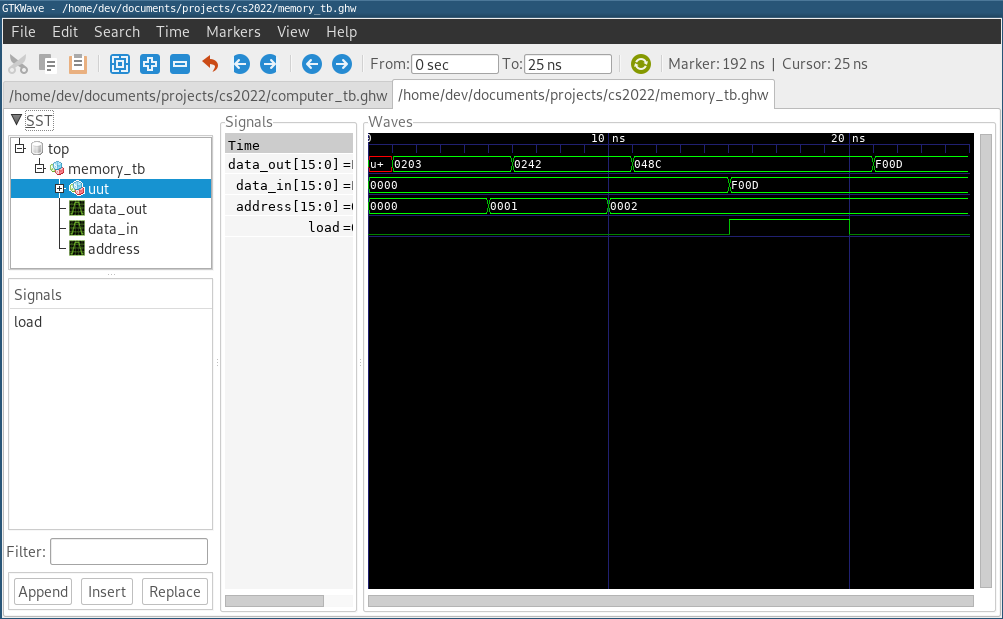
\includegraphics[width=\textwidth]{memory_tb}
	\caption{\mi{c}{memory} testbench results}
	\label{fig:memory}
\end{figure}

Figure~\ref{fig:memory} shows the simulation results of the 512x 16-bit word main memory.
\begin{itemize}
	\item After a short delay, setting the input address to \mi{c}{0} produces \mi{c}{0x203} (the first 
		instruction in memory) at \mi{c}{data_out}.
	\item Increasing the address shows the following instructions.
	\item Setting \mi{c}{data_in} and the load signal to high shows that the data at \mi{c}{0x2} is overwritten.
\end{itemize}

\newpage
\subsection{\mi{c}{control_memory}}
\begin{figure}[h!]
	\centering
	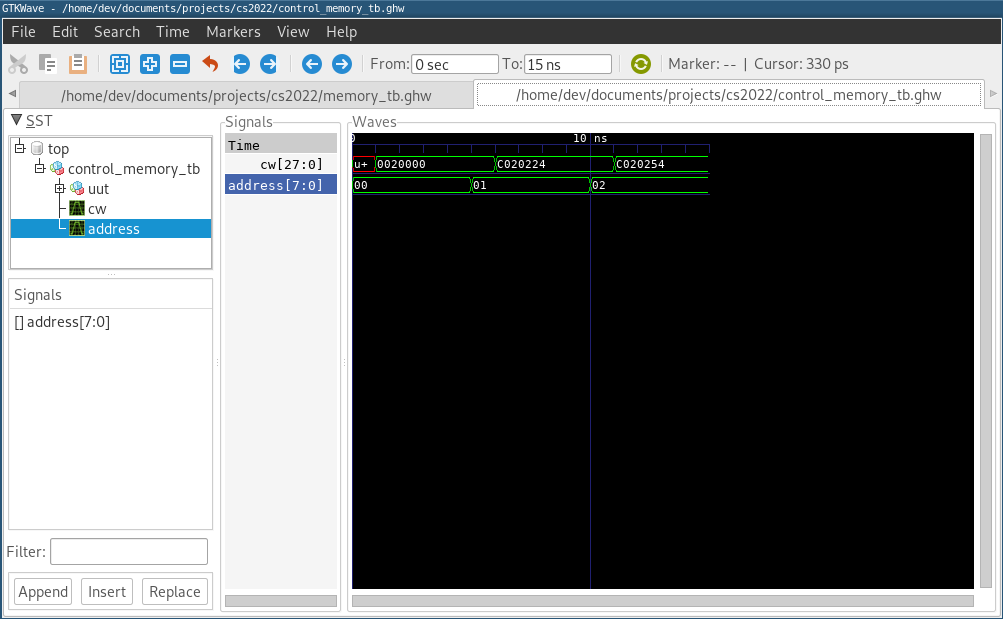
\includegraphics[width=\textwidth]{control_memory_tb}
	\caption{\mi{c}{control_memory} testbench results}
	\label{fig:cmemory}
\end{figure}

Figure~\ref{fig:cmemory} shows the simulation results of the 256x 28-bit word control (microcode) memory.

This memory just outputs the control word at the input address.

\newpage
\subsection{\mi{c}{flag_mux}}
\begin{figure}[h!]
	\centering
	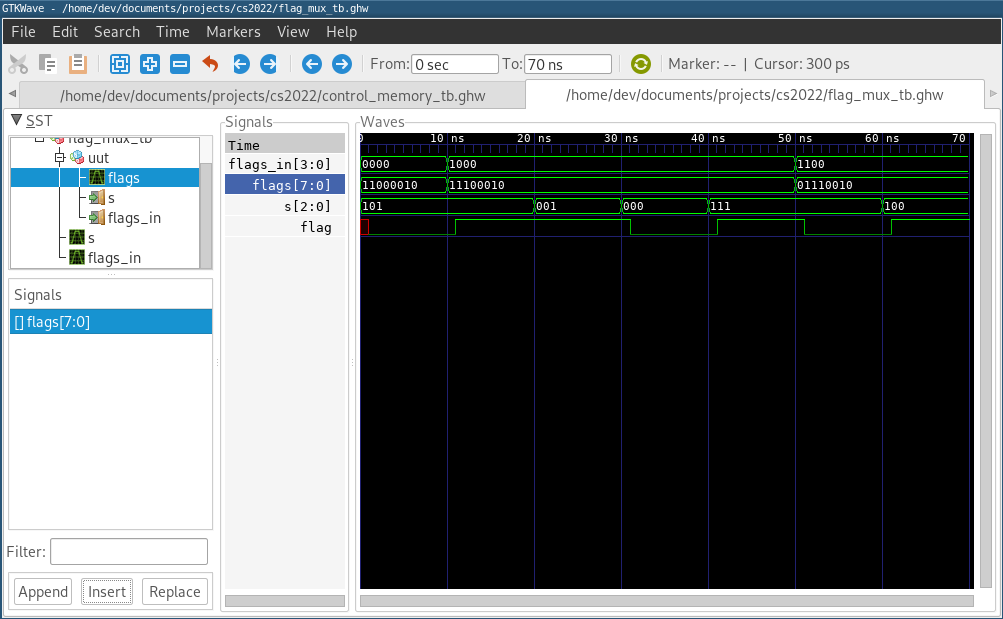
\includegraphics[width=\textwidth]{flag_mux_tb}
	\caption{\mi{c}{flag_mux} testbench results}
	\label{fig:fmux}
\end{figure}

Figure~\ref{fig:fmux} shows the simulation results of the flags mux, used to determine if the next CAR address 
should be loaded or incremented.

\mi{c}{flag} is the value of the bit selected from the internal \mi{c}{flags} vector by \mi{c}{s}.
\begin{itemize}
	\item \mi{vhdl}{flags(7) <= ~Z}
	\item \mi{vhdl}{flags(6) <= ~C}
	\item \mi{vhdl}{flags(5 downto 2) <= flags_in} (in the order \mi{c}{NZVC})
	\item \mi{vhdl}{flags(1) <= "1"} (constant)
	\item \mi{vhdl}{flags(0) <= "0"} (constant)
\end{itemize}

\newpage
\subsection{\mi{c}{car}}
\begin{figure}[h!]
	\centering
	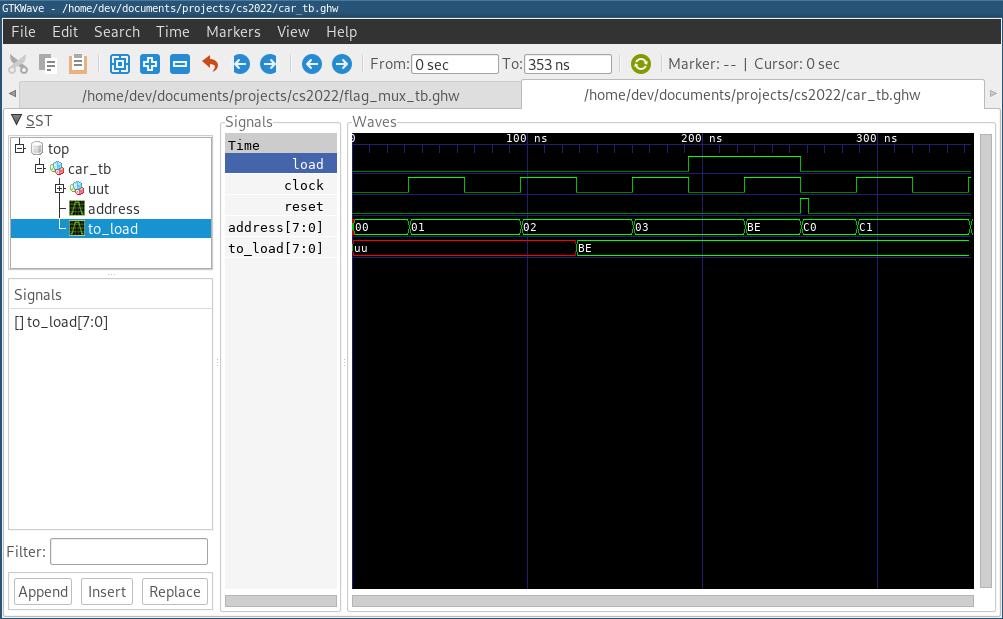
\includegraphics[width=\textwidth]{car_tb}
	\caption{\mi{c}{car} testbench results}
	\label{fig:car}
\end{figure}

Figure~\ref{fig:car} shows the simulation results of the Control Address Register (CAR).

\begin{itemize}
	\item When \mi{c}{load} is low, the CAR will increment its value by 1 on every clock.
		When high, it will load the input address on the next clock.
	\item Pulling \mi{c}{reset} high will set the address to \mi{c}{0xc0}, the address of the instruction fetch
		control word in the control memory.
\end{itemize}

\newpage
\subsection{\mi{c}{pc_extend}}
\begin{figure}[h!]
	\centering
	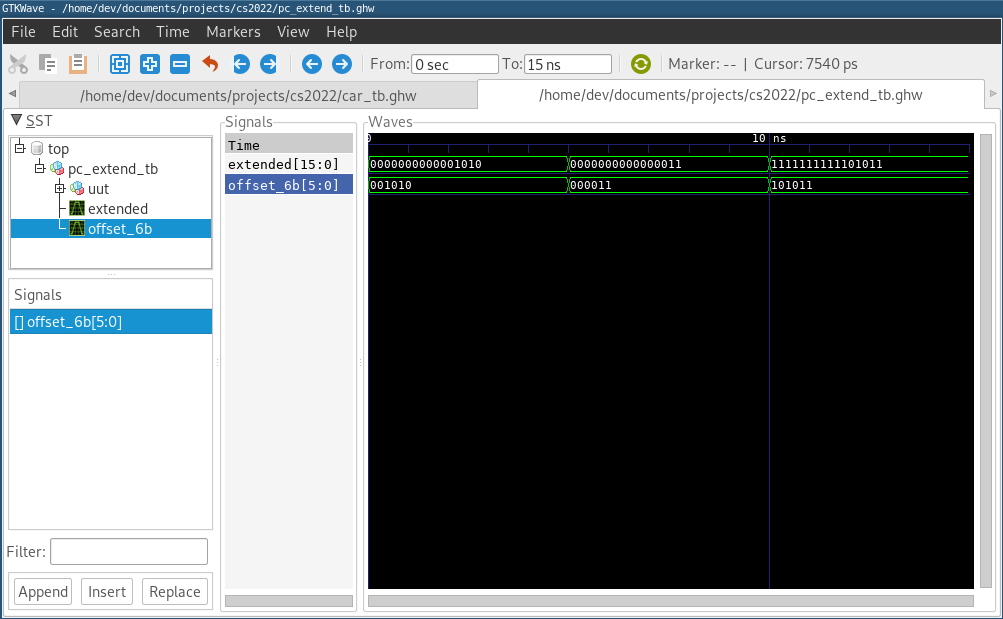
\includegraphics[width=\textwidth]{pc_extend_tb}
	\caption{\mi{c}{pc_extend} testbench results}
	\label{fig:pcext}
\end{figure}

Figure~\ref{fig:pcext} shows the simulation results of the Program Counter load extender.
This simply takes a 6 bit input (from the instruction register) and extends the top bit (sign) to 16 bits for 
input into the PC.

\newpage
\subsection{\mi{c}{pc}}
\begin{figure}[h!]
	\centering
	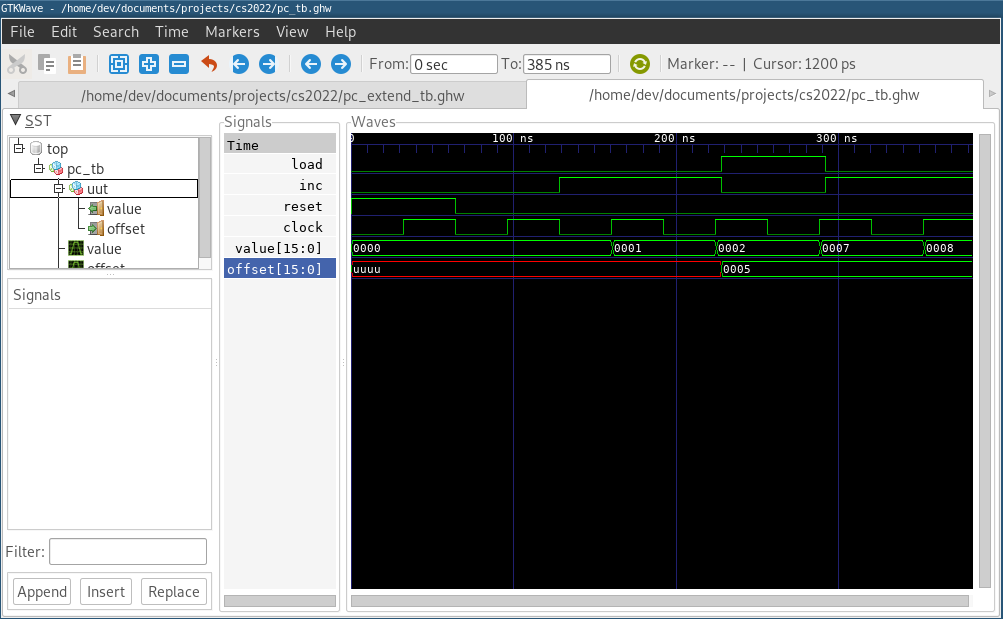
\includegraphics[width=\textwidth]{pc_tb}
	\caption{\mi{c}{pc} testbench results}
	\label{fig:pc}
\end{figure}

Figure~\ref{fig:pc} shows the simulation results of the Program Counter (PC).
\begin{itemize}
	\item When \mi{c}{inc} is high, the PC will increment its value on every clock.
	\item When \mi{c}{load} is high, the PC will add the input offset to its current value on the next clock.
\end{itemize}

\end{document}
# vim: nofoldenable
